\documentclass[numbers=noenddot,12pt,a4paper]{scrartcl}
\usepackage[greek,ngerman]{babel}
\usepackage[T1]{fontenc}
\usepackage[utf8]{inputenc}
\usepackage{fullpage}
\usepackage{libertine}
\usepackage{ziffer}
\usepackage{graphicx}
\usepackage{units}
\usepackage[infoshow]{tabularx}
\usepackage{amsmath}
\usepackage{amssymb}
\usepackage{wrapfig}
\usepackage{esint}
\usepackage{float}
\usepackage{wrapfig}
\usepackage[font=small]{caption}
\usepackage{subcaption}
\usepackage{lscape}
\usepackage{hyperref}

\renewcommand{\thefigure}{Abb. \arabic{figure}}

\captionsetup[wrapfigure]{name=}
\captionsetup[figure]{name=}
\newcommand{\degree}{^\circ}
\newcommand{\diff}{\textnormal{d}}
\newcommand{\tenpo}[1]{\cdot 10^{#1}}
\newcommand{\greek}[1]{\greektext#1\latintext}
\newcommand{\ix}[1]{_\text{#1}}
\newcommand{\imag}{\mathbf{i}}
\newcommand{\tilt}[1]{\mbox{\textit{#1}}}
\newcommand{\grad}[1]{\textit{grad}\left(#1\right)}
\newcommand{\divergenz}[1]{\textit{div}\left(#1\right)}
\newcommand{\euler}{\mathnormal{e}}
\newcommand{\fett}[1]{\textbf{#1}}

\title{Protokoll: Neodym-dotierter YAG-Laser} %TODO Name des Versuchs eintragen
\author{Philipp Hacker} %TODO Protokollschreiber unterstreichen
\date{\today}

\begin{document}
%\setcounter{page}{2}
%\setcounter{section}{1}
\maketitle
\begin{center}
Betreuer: U. Martens\\ %TODO Name des Betreuers eintragen
Versuchsdatum: 25.11.2014\\ %TODO Datum des Versuchs eintragen
\begin{table}[h]
\centering
Note: %TODO Gute Note erhalten :)
\begin{tabularx}{1.5cm}{|X|}
\hline \\ \\
\hline
\end{tabularx}
\end{table}
\end{center}
\vspace*{\fill}
\tableofcontents
\vfill
\newpage
\section{Einleitung}
1964 wurde in den Bell Laboratories (New Jersey, USA) von \tilt{L. Van Uitert} und \tilt{J. E. Geusic} ein Festkörper-Laser auf Grundlage eines Neodym-dotierten Yttrium-Aluminium-Granat-Kristalls entwickelt. Dieser hatte den Vorteil, dass er bei relativen hohen Ausgangsleistungen von einigen hundert $\unit{MW}$ im gepulsten Betrieb einen Laserstrahl mit einer geringen Wellenlänge (hauptsächlich $\unit[1064]{nm}$) aussendet. Der Nd:YAG kann sowohl mit Lichtquellen kontinuierlicher Spektren oder einer Laser-Diode angeregt werden. Diese haben, bei einer Pump-Wellenlänge von $\unit[808]{nm}$, einen Wirkungsgrad von $\sim0,7\,$. Die Effizienz des Lasers steigert sich dadurch auf bis zu $50\%$.\\ Aufgrund der vielen Möglichkeiten, Halbleiterstrukturen zu verändern, kann man die Anregung nur eines Übergangs innerhalb der zum Pumpen genutzten Diode realisieren. Bei geeigneter Stabilisierung der Parameter Temperatur und Pumpstrom lässt sich somit eine äußerst geringe Frequenzbandbreite des Lasers einstellen. \\
In diesem Versuch soll sich auf die Untersuchung der Eigenschaften des Laser-Mediums \tilt{Nd:YAG} und der Leistung in Abhängigkeit der Erregung und des Aufbaus konzentriert werden. 
\newpage
\section{Grundlagen}
\subsection{Festkörper-Laser}\label{subsec:fklaser}
Diese Laser (\tilt{\textbf{L}ight \textbf{A}mplification} by \textbf{S}timulated \textbf{E}mission of \textbf{R}adiation), welche aus kristallinen oder amorphen Festkörpern bestehen, können die höchsten Ausgangsleistungen bei den geringsten Impulslängen aller Laser erreichen. Grundsätzlich besteht das Laser-Medium aus einem Kristall (Träger-Medium; hier: YAG), welcher wiederum mit einer bestimmten Dotierung versehen ist (aktives Medium; hier: Neodym). Der entspiegelte Festkörper befindet sich zwischen einem absolut reflektierenden \mbox{(Reflexionskoeffizient $R=1$)} und teildurchlässigen ($R<1$, Transmissionskoeffzient $T>0$) Spiegel, dem sogenannten Resonator. Ein weiterer Bestandteil des Aufbaus ist die Pumplichtquelle (siehe \ref{subsec:optpump}). Sie regt das Laser-Medium mit ihrem elektromagnetischen Strahlungsfeld auf atomarer Ebene an und sorgt damit für dessen Eigenfluoreszenz. Im Resonator können zusätzlich noch andere optische Bauteile wie z.Bsp. Filter eingebaut werden, welche das Ausgangsspektrum oder die erregten Moden verändern. Diese Laser können auf 2 Arten betrieben werden: kontinuierlich -- Pumplicht und Laser-Licht werden ohne vorgegebene Periode emittiert -- und gepulst -- einerseits kann das Pumpen durch getaktete Lichtimpulse erfolgen und andererseits der Resonator des Lasers verändert werden.\\ Die Ausgangspunkte der Übergänge in den Ionen der Dotierung, welche durch das Pumpen induziert werden, sind  nur d- bzw. f-Orbitale. Da diese keine gemeinsamen Elektronen-Wellenfunktion mit dem umgebenden Kristall haben, d.h. nicht an der Bindung beteiligt sind, können die Eigenschaften des Träger-Mediums in Hinblick auf das Verhalten des Lasers vernachlässigt werden.\\
Identifiziert man die Energie des Niveaus, welches angeregt werden soll, über die Planck-Konstante mit einer Frequenz $f$ bzw. Wellenlänge $\lambda$, so kann man die nötige Pumplichtfrequenz/-wellenlänge aus der Differenz der Energien von angehobenem und relaxiertem Zustand erhalten. Überlegt man nun, wie die Besetzungsdichten der Zustände sich unter dem Pumpprozess verhalten, so erkennt man schnell, dass das nicht-angeregte Energieniveau an Teilchen unweigerlich verarmen wird. Dies kann nur unter steter Energiezufuhr erzwungen werden, da es dem Streben nach maximaler Entropie eines Systems widerspricht (Besetzungsinversion, siehe \ref{subsec:besetzinv}).
\subsection{Dioden-Laser}\label{subsec:dlaser}
Am Übergang eines p-dotierten zu einem n-dotierten Halbleiterbauelement kommt es zur Rekombination von positiv geladenen "`Löchern"' und Elektronen. Aufgrund der Energiedifferenzen in den Bändern (Überlapp der Wellenfunktion aller Teilchen) der beiden Halbleiterschichten kommt es zur Emission von Photonen. Durch das Anlegen einer äußeren Spannung an die aktive pn-Zone fließen Ladungsträger aus dem n-dotierten in den p-dotierte Halbleiter. Wird der Strom groß genug, d.h. größer als der für den Dioden-Laser charakteristische Schwellenstrom $I\ix{th}$, so stellt sich eine Besetzungsinversion (siehe \ref{subsec:besetzinv}) zwischen den beiden Schichten ein.
\\Laserdioden unterscheiden sich somit von herkömmlichen Lasern. Einerseits wird nur ein einziges Energieniveau angeregt und die Teilchen, welche dieses besetzen, sind unabhängig voneinander. Andererseits liegt die Ausgangsleistung nur bei einigen $\unit{mW}$. Da die Besetzung der Bänder dem thermodynamischen Gleichgewicht nach \tilt{Fermi-Dirac} folgt, ist die Lichtwellenlänge der Laserdiode keine scharf definierte, sondern entspricht einer Distribution von Energien der am Übergang zwischen den Schichten beteiligten Teilchen. Außerdem ist bei Laserdioden zu beachten, dass der Resonator durch die reflektieren/transmittierenden Eigenschaften der zum Einsatz kommenden Halbleiter gegeben ist. Er hat in etwa die Dimension der Wellenlänge des \mbox{Laserdioden-Lichts}.\\Wie bei Halbleiter-Kristallen üblich, hängen auch die Eigenschaften der Laserdioden stark von der Intensität des Ladungsträgerstroms und der Temperatur ab. Wird nun eine einzige Wellenlänge, zum Beispiel zum optischen Pumpen (siehe \ref{subsec:optpump}) eines Laser-Mediums benötigt, so müssen Temperatur und Diodenstrom genauestens kontrolliert und geregelt werden. Offensichtlich nimmt die Laser-Lichtwellenlänge mit sinkender Temperatur ab (siehe \ref{img:lambdat}), da in diesem Fall sich die Energiebandlücke vergrößert und somit auch die Energie, welche beim Übergang eines Teilchens frei wird. Hinzu kommt, das sich Resonatorgröße und -eigenschaften mit der Temperatur verändern. Deswegen können auch die ausgesendeten Photonen oberhalb bzw. unterhalb bestimmter Temperaturen keine stehenden Wellen mehr ausbilden. In diesen Fällen findet die Anregung anderer Moden statt, was wiederum eine Änderung der Wellenlänge des Lichts zur Folge hat (siehe \ref{img:stromt}).
\begin{figure}[H]
	\begin{subfigure}[htbp]{0.45\textwidth}
		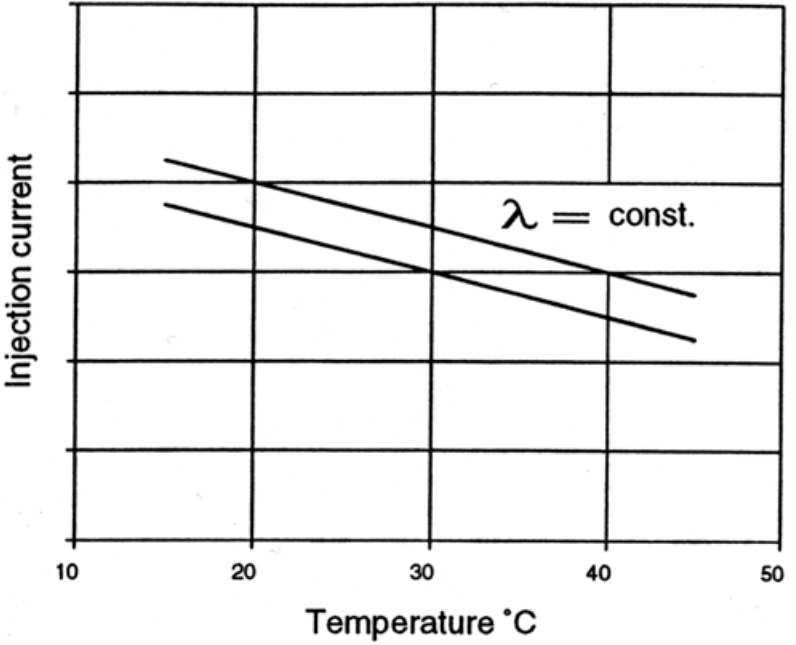
\includegraphics[width=\textwidth]{stromT.png}
		\caption{Diodenstrom (\tilt{injection current}) über der Temperatur (\tilt{Temperature}) für konstante Wellenlängen $\lambda$}\label{img:stromt}
	\end{subfigure}
	\hspace{0.5cm}
	\begin{subfigure}[htbp]{0.45\textwidth}
			\vspace{-0.9cm}
		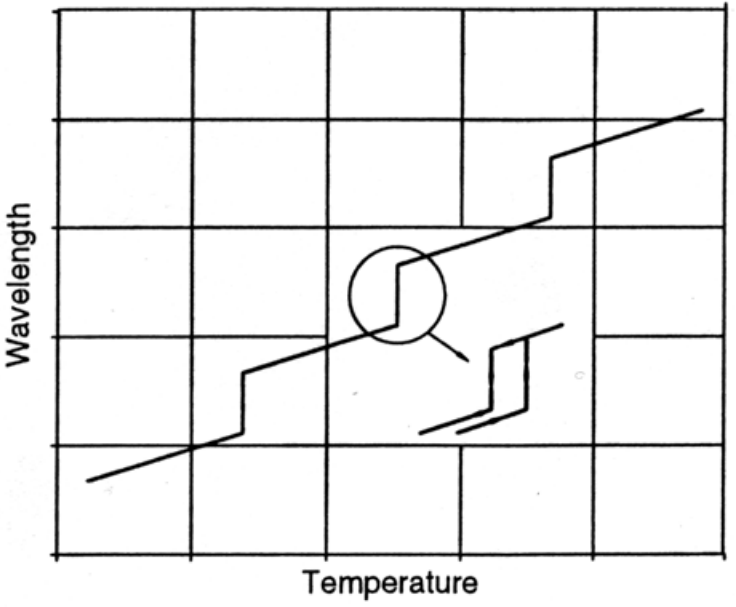
\includegraphics[width=\textwidth]{lambdaT.png}
		\caption{Wellenlänge (\tilt{Wavelength}) des Diodenlasers über Temperatur (\tilt{Temperature})}\label{img:lambdat}
	\end{subfigure}
	\caption{Charakteristische Geraden einer Laser-Diode}
	\label{img:diodechar}
\end{figure}
\subsection{Emission und Besetzungsinversion}\label{subsec:besetzinv}
Ein Medium, welches elektromagnetischer Strahlung ausgesetzt ist, kann Photonen bestimmter Energien aufnehmen und abgeben. Diese Vorgänge heißen Absorption und Emission. Im ersten Fall ist es so, dass die Energie eines Teilchens (Elektronen oder Nukleonen) zum Übergang von einem energetisch niedrigeren in einen höheren Zustand gerade durch ein Photon gestellt wird. Der Vorgang der Emission kann sich auf zwei Arten vollziehen. Einerseits kann ein angeregtes Teilchen, unter der Abgabe der Energiedifferenz der Niveaus in Form eines Photons, in seinen Ausgangszustand zurück relaxieren. Andererseits kann durch das äußere Strahlungsfeld ein Teilchen zur Verringerung seiner Energie induziert werden. Diese entspricht gerade der des stimulierenden Photons. Das Ergebnis der stimulierten Emission sind somit 2 Photonen gleicher Energien.\\
Ist die Änderung der Zustandsverteilungen $N\ix{i}(t)$ proportional zur ursprünglichen Anzahl $N\ix{i}(t\ix{0})$ und der Energiedichte des Strahlungsfeldes $\rho\ix{ext}$, so lässt sich für alle drei Vorgänge zwischen den Niveaus $i$ und $j$ schreiben
\begin{align}
	\text{Absorption :} \,\, \frac{\diff N\ix{i}(t)}{\diff t}=&-B\ix{ij}\cdot N\ix{i}(t\ix{0})\cdot \rho\ix{ext} \label{eq:absorp}\\
	\text{Emission :} \,\, \frac{\diff N\ix{j}(t)}{\diff t}=&\frac{\diff N\ix{j, spo.}}{\diff t}+\frac{\diff N\ix{j, stim.}}{\diff t}=\left(-B\ix{ji}\cdot \rho\ix{ext}+-A\ix{ji}\right)\cdot N\ix{j}(t\ix{0}) \label{eq:emiss} \,\,.
\end{align}
($B\ix{ij}$, $A\ix{ij}$ - Einsteinkoeffizienten des Übergangs $i\rightarrow j$) \\
Man sieht an Gl. (\ref{eq:emiss}) sofort, das die spontane Emission einem Zerfallsgesetzt mit der Halbwertszeit $\tau=1/A\ix{ji}$ entspricht.\\
Folgen die Besetzungszahlen der diskreter Energieniveaus, welche an Absorption/Emission beteiligt sind, einer statistischen Temperaturverteilung\\ (\tilt{Boltzmann-Statistik}, \tilt{Fermi-Dirac-Statistik}), so besteht eine Besetzungsinversion, wenn die Verhältnisse der Teilchenzahlen in den jeweiligen Zuständen gerade umgekehrt bezüglich der gewählten Verteilung sind.\\
Sei $E\ix{2}$ mit dem statistischen Gewicht $g\ix{2}$ ein energetisch höheres Niveau als $E\ix{1}$ mit $g\ix{1}$, so folgt für die Gleichverteilung mit der Boltzmann-Statistik bei der Temperatur $T$ die Dichte der Teilchen im Zustand $E\ix{2}$ (analog $E\ix{1}$)
\begin{align}
	N\ix{2}=&N\ix{1}\cdot\frac{g\ix{2}}{g\ix{1}}\cdot\euler^{-\frac{E\ix{2}-E\ix{1}}{k\ix{B}T}} \,. \label{eq:dichte} \\
	\text{Inversion für :} \,\, N\ix{2}>&\frac{g\ix{2}}{g\ix{1}}\cdot N\ix{1} \label{eq:invers}
	\end{align}
Wie bereits angesprochen (in \ref{subsec:fklaser} ) kann eine Besetzungsinversion ohne äußere Erregung nicht realisiert werden, wie Gl. (\ref{eq:dichte}) und (\ref{eq:invers}) mit $E\ix{2}-E\ix{1}>0$ verdeutlicht. Das heißt, dass ausgewählte, höhere Niveaus durch sogenanntes Pumpen (siehe \ref{subsec:optpump}) mit diskreten Energien des Erregungsspektrums stärker besetzt werden können. Man muss jedoch beachten, dass ein sehr kleines Frequenzband ($\delta\nu\approx\unit[10]{Hz}$) zur Anregung eines Zustandes zuständig ist. Dies ist Folge der Unschärfe des Impulses der Pump-Photonen (Gl. (\ref{eq:breite}) nach \tilt{Heisenberg}, 1927) und der Doppler-Verbreiterung (Gl. (\ref{eq:doppler}) nach \tilt{Doppler}, 1842).
\begin{align}
	2\pi\delta\nu=\frac{1}{\tau}=A\ix{ji} \label{eq:breite}\\
	\delta\nu=\frac{\overline{\nu}}{c}\sqrt{\frac{8k\ix{B}T\ln\left(2\right)}{m}} \label{eq:doppler}
\end{align}
\pagebreak
\subsection{Optisches Pumpen}\label{subsec:optpump}
\begin{wrapfigure}[15]{ro}{0.45\textwidth}
	\vspace{-0.75cm}
	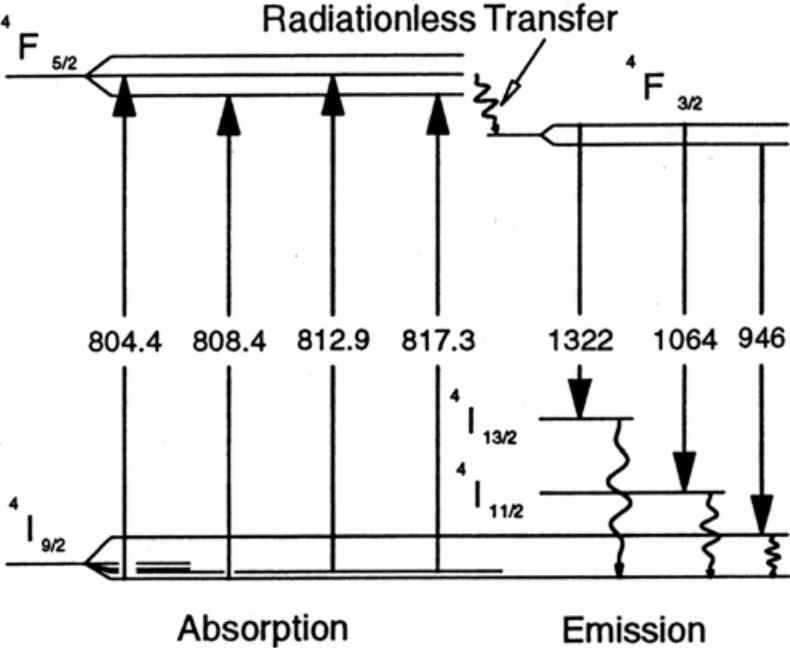
\includegraphics[width=0.45\textwidth]{uebergaenge.png}
	\caption{Termschema mit strahlungsloser Relaxation (\tilt{Radiationless Transfer}) des Nd:YAG}\label{img:übergänge}
\end{wrapfigure}
Licht, welches auf ein Medium abgestrahlt wird, ruft eine Anregung hervor und verändert damit die Besetzungen der Zustände, welche mit der Energie der Photonen korrespondieren. Die Absorption (siehe \ref{subsec:besetzinv}) der Teilchen findet nur bei diskreten Frequenzen bzw. Wellenlängen auf den atomaren Energieniveaus der Elektronen der Hülle statt, da die Photonen nur bestimmte Energien $E=\hbar\omega\,$ transportieren. Optisches Pumpen ist somit das Verfahren der spektralen Anregung eines diesbezüglich aktiven Mediums unter Ausnutzung der Besetzungen der Zustände (nach \tilt{Boltzmann}) und der Eigenschaften der Elektronen in den Hüllen. \ref{img:übergänge} zeigt die Übergänge in den Zuständen des Nd:YAG für die jeweiligen Wellenlängen.
\subsection{Der Nd:YAG-Laser}\label{subsec:ndyag}

Der Nd:YAG-Laser wird mit Licht einer Wellenlänge $\sim\unit[810]{nm}$ gepumpt und emittiert hauptsächlich bei $\unit[1064]{nm}$ \ref{img:4niv} und \ref{img:übergänge} stellen das Prinzip der, bei gegebener Dotierung und Pump-Lichtquelle induzierten Übergänge im Laser-Medium dar. Dabei handelt es sich um ein sogenanntes 4-Niveau-System. \\
Von 1 zu 4: das Pumplicht regt den im Kristall thermisch besiedelten Zustand in einen höheren an. Von 4 zu 3: die sehr schnelle, strahlungslose Relaxation verhindert den Zerfall in den Grundzustand. Diese geschieht meist wegen mechanischen Wechselwirkungen, wie zum Beispiel Stößen. Von 3 zu 2 und zurück: die relevanten Übergänge für das Laser-Licht -- hier finden spontane und induzierte Emission statt, wobei jedoch beide beteiligten Zustände keine thermische Besetzung aufweisen. Unter Umständen kann sogar aus dem Niveau 2 in 3 eine durch Absorption induzierte Anregung stattfinden. Von 2 zu 1: die Relaxation, welche den Ausgangszustand wiederbesiedelt.\\
Die charakteristischen Linien der besprochenen Absorptionsübergänge sind in \ref{img:yes} über der Temperatur der Laser-Diode dargestellt. Die dort gezeigten Absorptionspeaks entsprechen gerade einer Energie des Pumplichts und somit einem Übergang im Nd.
\begin{figure}[H]
	\centering
	\begin{subfigure}[htbp]{0.49\textwidth}
	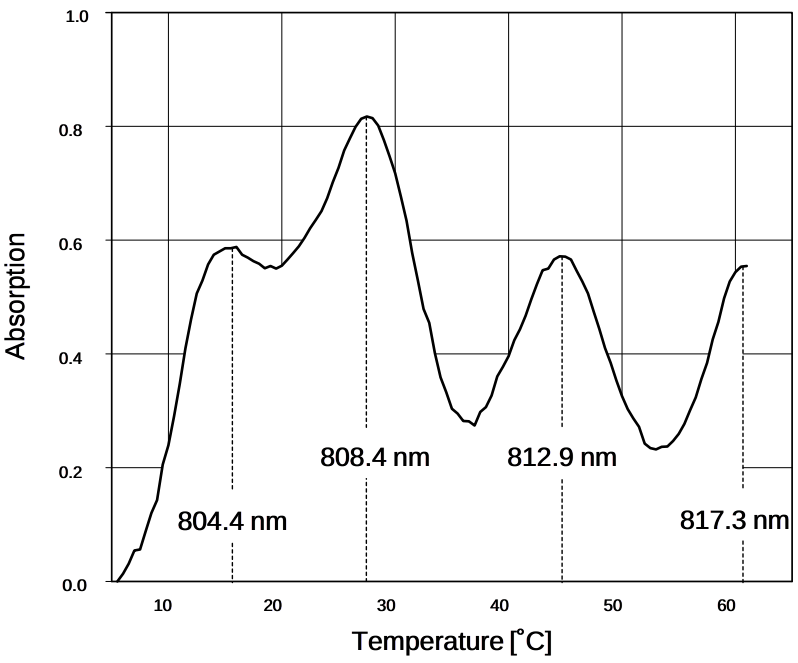
\includegraphics[width=\textwidth]{yes.png}
	\caption{Absorption des Nd:YAG in Abhängigkeit der Laser-Diodentemperatur}\label{img:yes}
	\end{subfigure}
\begin{subfigure}[htbp]{0.49\textwidth}
	\vspace{-0.3cm}
	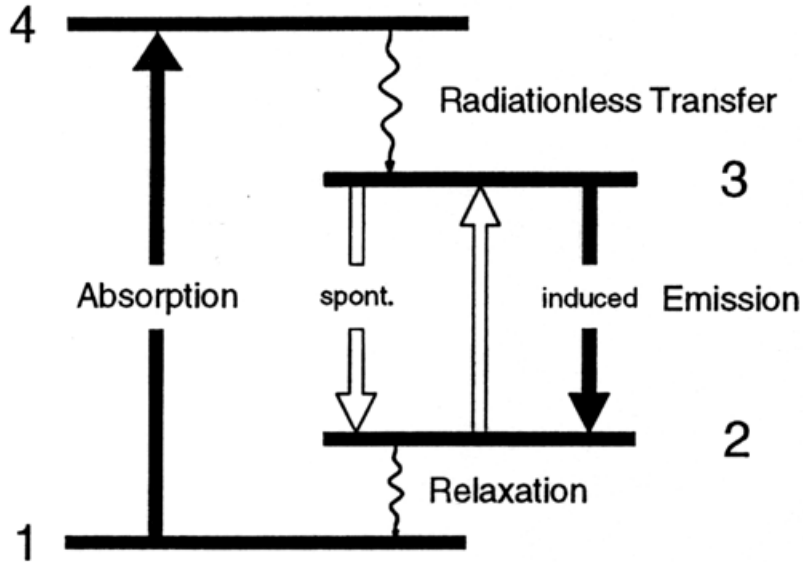
\includegraphics[width=\textwidth]{vierniveau.png}
	\vspace{0.3cm}
	\caption{4-Niveau-System des Nd:YAG-Lasers}\label{img:4niv}
\end{subfigure}
\caption{Schemata für den Nd:YAG-Laser}
\end{figure}
\pagebreak
\section{Durchführung}\label{sec:durch}
Den Aufbau des Lasers zeigt \ref{img:aufbau}. Die Laser-Diode \fett{A}, deren Lichtstrahl durch Feinjustierung mit Schrauben nach Bedarf gerichtet werden kann, wird bereits mit Kühleinheit und Temperatursensor montiert. \fett{B} ist ein Kollimator. Dieser parallelisiert das stark divergente Laser-Licht, welches aus der pn-Schicht der Diode austritt. \fett{C} ist ein Linsensystem zur Fokussierung auf das Laser-Medium. Die Einheiten \fett{D}, \fett{K} und \fett{E} bilden den Resonator des Lasers. In \fett{D} selbst ist der stabförmige Nd:YAG-Kristall verbaut. Dieser ist in der Eingangsrichtung für die Wellenlänge $\unit[1064]{nm}$ und in der Ausgangsrichtung für $\unit[532]{nm}$ (1.Oberwelle) stark reflektierend. Das Innere der Module des Resonators ist ebenfalls beschichtet, wodurch der Leistungsverlust minimiert werden soll. Der Strahlengang im Resonator kann wiederum mit Schrauben zur Justierung optimiert werden. Einheit \fett{F} ist ein optischer Filter, welcher zur Absorption bestimmter Spektralbereiche genutzt wird. Mit \fett{G} liegt unser Messsensor in Form eines Photodetektors mit Verstärker vor, welcher schlichtweg in ein Oszilloskop \fett{O} oder ein Multimeter eingespeist wird. \fett{H} in die Steuer-Einheit des Versuchs. Sie zeigt die Temperatur der Pumplichtquelle an und ermöglicht die Variation des Diodenstroms. Weiterhin kann ein kontinuierlicher oder gepulster Modus eingestellt werden, wobei hier noch zwischen interner und der externen Taktung \fett{M} (Frequenzgenerator o.ä.) unterschieden wird.
\begin{figure}[H]
	\centering
	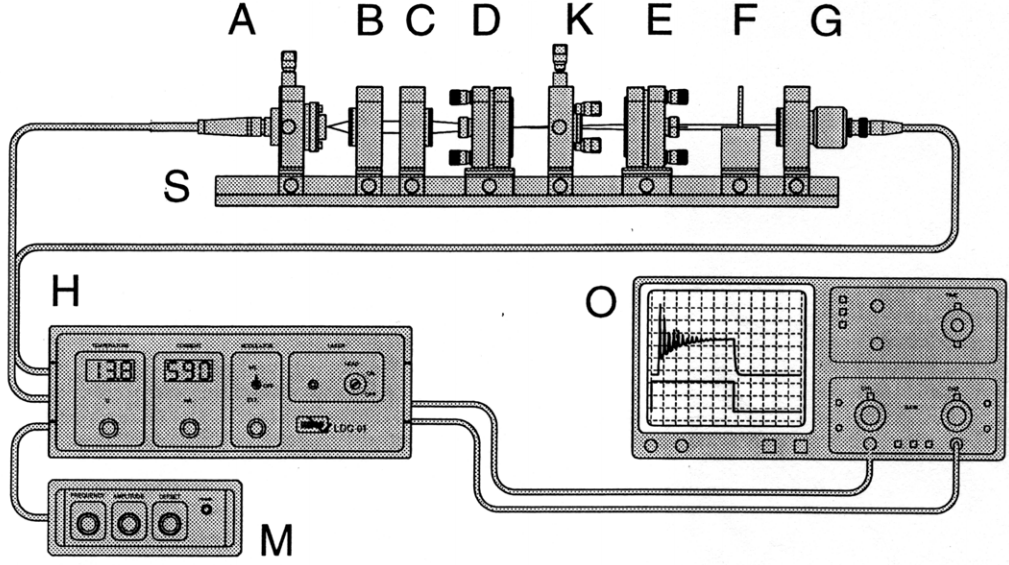
\includegraphics[width=0.8\textwidth]{aufbau1.png}
	\caption{Gesamter Aufbau des Versuchs zum Nd:YAG-Laser}\label{img:aufbau}
\end{figure}
Eingangs wird der charakteristischer Zusammenhang von Diodenstrom und Ausgangsleistung der genutzten Laserdiode untersucht. Bei konstanter Temperatur wird hierfür $I$ im erlaubten Bereich (ohne die Diode zu beschädigen) variiert. Dabei sind nur die Module \fett{A}, \fett{B} und \fett{G} im Strahlengang. Den Messwert liefert der Photo-Detektor.\\
Anschließend wurde das Fluoreszenzspektrum des Nd:YAG-Stabes aufgenommen. Dafür wurde die Temperatur der Laser-Diode verändert. Die Einheiten \fett{A}, \fett{B}, \fett{C}, \fett{G} und \fett{D} werden verbaut.\\
Stellt man nun in \fett{H} den Betrieb auf gepulst, so kann man oszillographisch mit \fett{O} die mittlere Lebensdauer/Halbwertszeit des dominanten Emissionsübergangs bestimmen. Dies wird für den $^{4}F\ix{3/2}$-Zustand des Nd:YAG getan (siehe \ref{img:übergänge}).\\
Anschließend wird der gesamte Aufbau des Versuchs-Lasers realisiert und optimiert. Dieser wird wiederum unter Veränderung der Pumpleistung ausgemessen.\\
Zum Schluss Filtert man den Laser-Strahl bis auf seine 1. Oberwelle bei $\unit[532]{nm}$ und untersucht dessen Leistungsabhängigkeit.
\pagebreak
\section{Auswertung}\label{sec:auswert}
\subsection{Aufgabe 1}
In der Messaufgabe 1 sollte die Ausgangsleistung $P\ix{D}$ der Diode in Abhängigkeit von dem durch sie fließenden Strom $I\ix{D}$ untersucht werden. Man erwartete, wie zuvor angemerkt, das ab einem gewissen Schwellenstrom $I\ix{th}$ die Strahlungsleistung erheblich anwachsen würde, da ab diesem Strom Besetzungsinversion eintritt.\\
Um einen Zusammenhang über den gemessenen Strom $I\ix{Ph}$ und die Strahlungsleistung $P\ix{Ph}$ zu erhalten, benutzten wir proprietäre Messkurven des Herstellers des Photodetektors (siehe Quellen). Mittels einer linearen Näherung für die Kennlinie unter $\lambda=\unit[1064]{nm}$ erhielten wir somit
\begin{align}
	P\ix{Ph}\left(I\ix{Ph}\right)=\unit[0,1175(12)]{\frac{mW}{\mu A}}\cdot I\ix{Ph}-\unit[0,16589(91)]{mW} \,
\end{align}
Hat man Kenntnis über die Strahlungsleistung in Abhängigkeit des Detektor-Stroms, so kann man die gewonnen Messdaten in Form von \ref{img:diodleistung} aufbereiten. Gut zu erkennen ist der erwartete lineare Zusammenhang (siehe Versuchsanleitung) und der Ordinatenabschnitt, welcher den Schwellenstrom $I\ix{th}$ darstellt. Dieser ergab sich zu $I\ix{th}=\unit[168,36653(59)]{\mu A}$.
\begin{figure}[H]
	\centering
	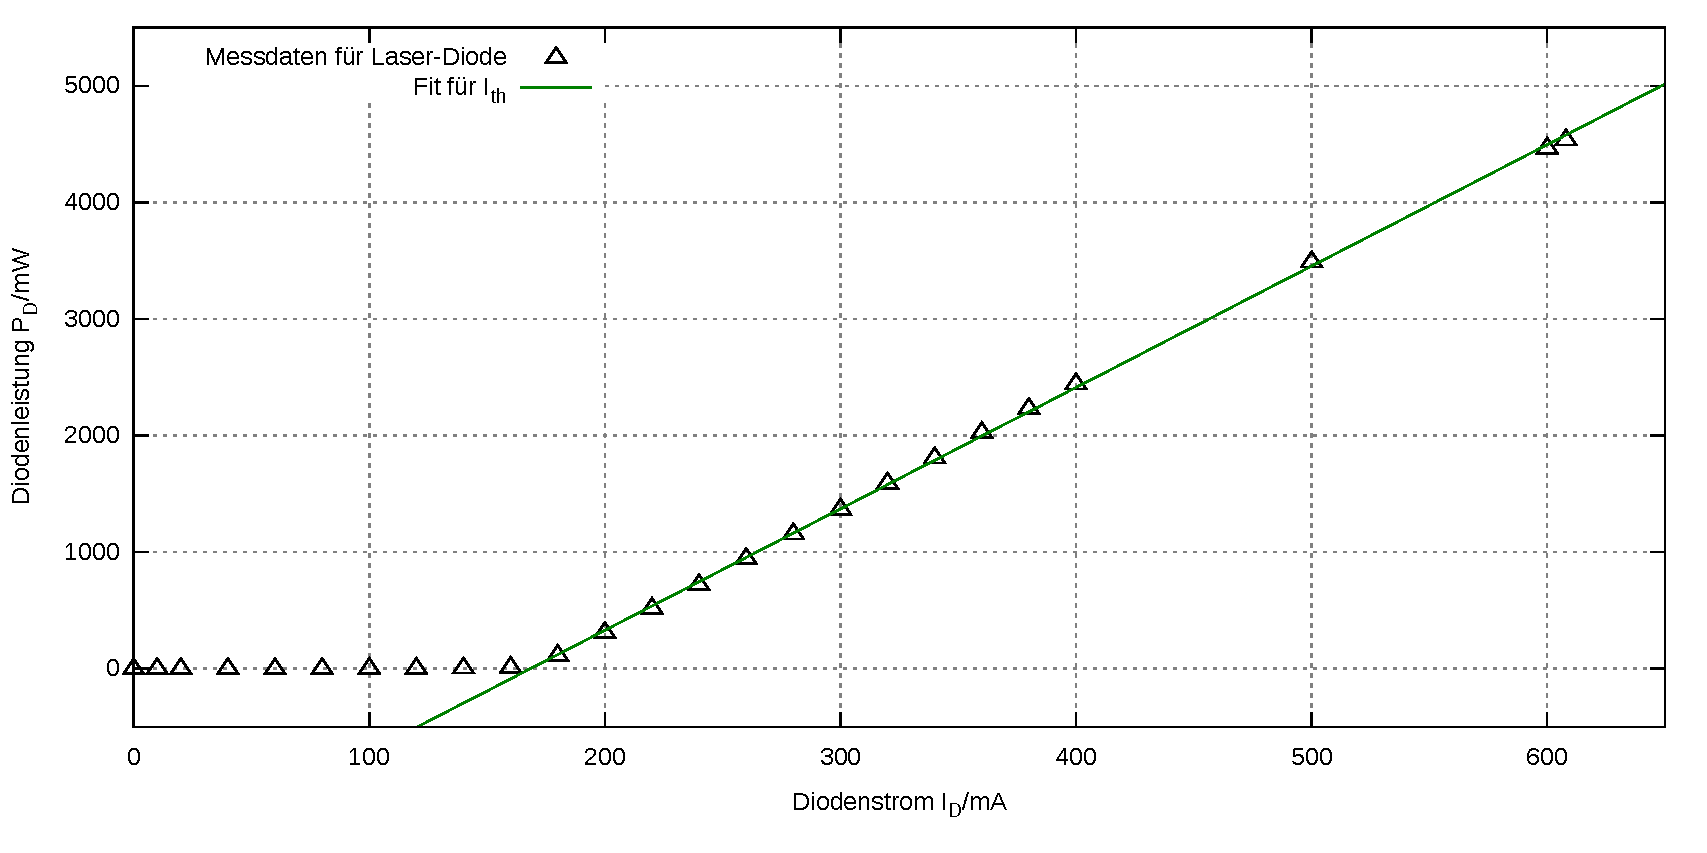
\includegraphics[width=\textwidth]{messwerte/diodenleistung.pdf}
	\caption{Ausgangsleistung der Diode (eigene Kennlinie) und Fit zur Bestimmung von $I\ix{th}$}\label{img:diodleistung}
\end{figure}
\subsection{Aufgabe 2}
In Messaufgabe 2 sollte das Fluoreszenz des Nd:YAG aufgenommen werden.\\
Aus den Grundlagen \ref{subsec:dlaser} wissen wir, das für den Betrieb mit einem linearen Diodenstrom-Diodentemperatur-Verlauf Licht mit festen Wellenlängen abgestrahlt werden kann. Deswegen wird hierbei für einen eingestellten Strom die Temperatur der Diode verändert, um so ihr Spektrum zu durchlaufen. Pumpt man so den Laser-Kristall mit den verschiedenen Frequenzen, so lässt sich dessen Fluoreszenzspektrum aufnehmen.\\
Leider wurde keine Referenzmessung durchgeführt, weswegen man nur mit den Werten für die Strahlungsleistung durch den Nd:YAG-Stab verbleibt (siehe \ref{img:shit}). Der Vergleich mit den Erwartungen aus \ref{img:yes} ermöglicht ebenso keinen Rückschluss auf die Güte der Messung.
\begin{figure}[H]
	\centering
	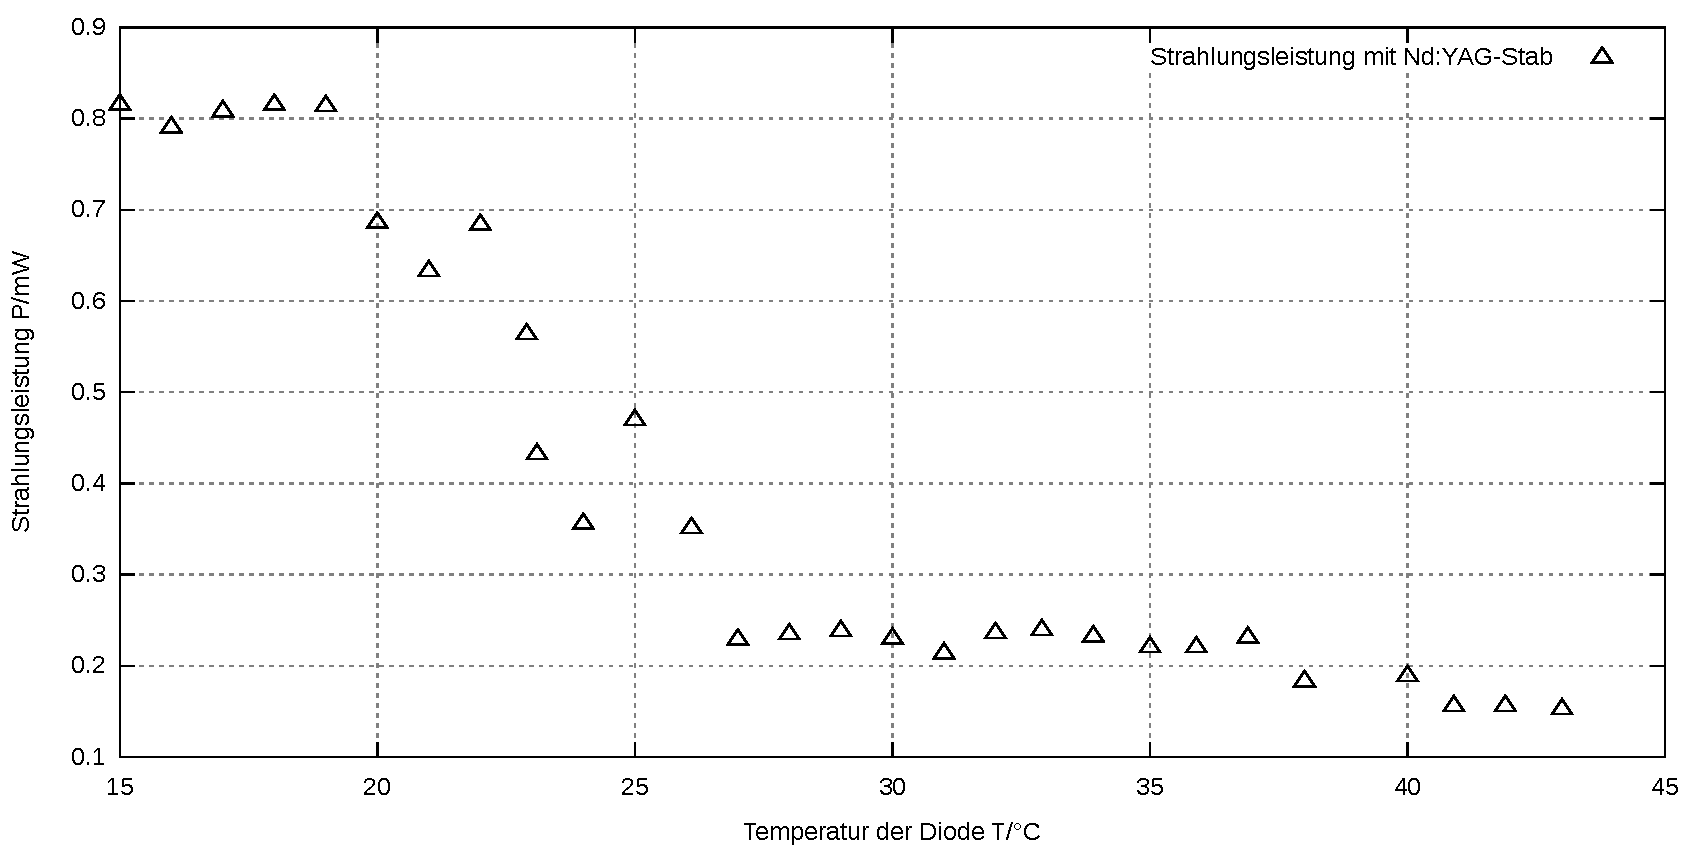
\includegraphics[width=\textwidth]{messwerte/fluoreszenz.pdf}
	\caption{Verbleibende Strahlungsleistung nach Durchgang des Nd:YAG-Stabes in Abhängigkeit von $T$}\label{img:shit}
\end{figure}
\subsection{Aufgabe 3}
Die Lebensdauer des Zustandes $^{4}F_{3/2}$, welcher Licht der Wellenlänge $\unit[1064]{nm}$ aussendet, liegt im Bereich von $\unit[250]{\mu s}$. Diese Zeit muss nach Anregung verstreichen, damit die Intensität dieser Linie im Spektrum gerade auf das $1/e$-fache abgesunken ist. An diesem Abfall ist nur die spontane Emission beteiligt, weswegen ein Zerfallsgesetz bspw. für die Zahl dieser angeregten Zustände angenommen werden kann. Mit Hilfe des Oszilloskops konnte, bei gepulstem Betrieb der Laser-Diode, der Intensitätsverlauf der durch den Nd:YAG gelangten Strahlung beobachtet werden. Ein Filter absorbiert hier zusätzlich die Signale, welche irrelevant für diese Messung sind.\\
Die Zeitauflösung des Signals erhielten wir durch das \tilt{triggern} mit dem Pulstakt der Laser-Diode. So ergab sich die gesuchte Lebensdauer zu $4,4\cdot\unit[50]{\mu s}=\unit[220]{\mu s}$. Dieser Wert liegt im Bereich des erwarteten.
\subsection{Aufgabe 5 und 6}
Hierbei wurde die Leistung des Nd:YAG-Lasers, aufgelöst nach dem Pump-Diodenstrom gemessen. Durch die Kenntnis der Abhängikeit von Strom durch die Laser-Diode und Pumpleistung kann ein Bezug zwischen $P\ix{Nd:YAG}$ und $P\ix{D}$ hergestellt werden. Hierfür ist ein, in großen Bereichen linearer Zusammenhang zu erwarten. In der Nähe der Ordinate sollte eine Abweichung auftreten, da nun der Strom, für welchen Besetzungsinversion in der Diode \underline{und} im Nd:YAG eintritt verschieden von dem bereits diskutierten $I\ix{th}$ ist.
\begin{figure}[H]
	\centering
	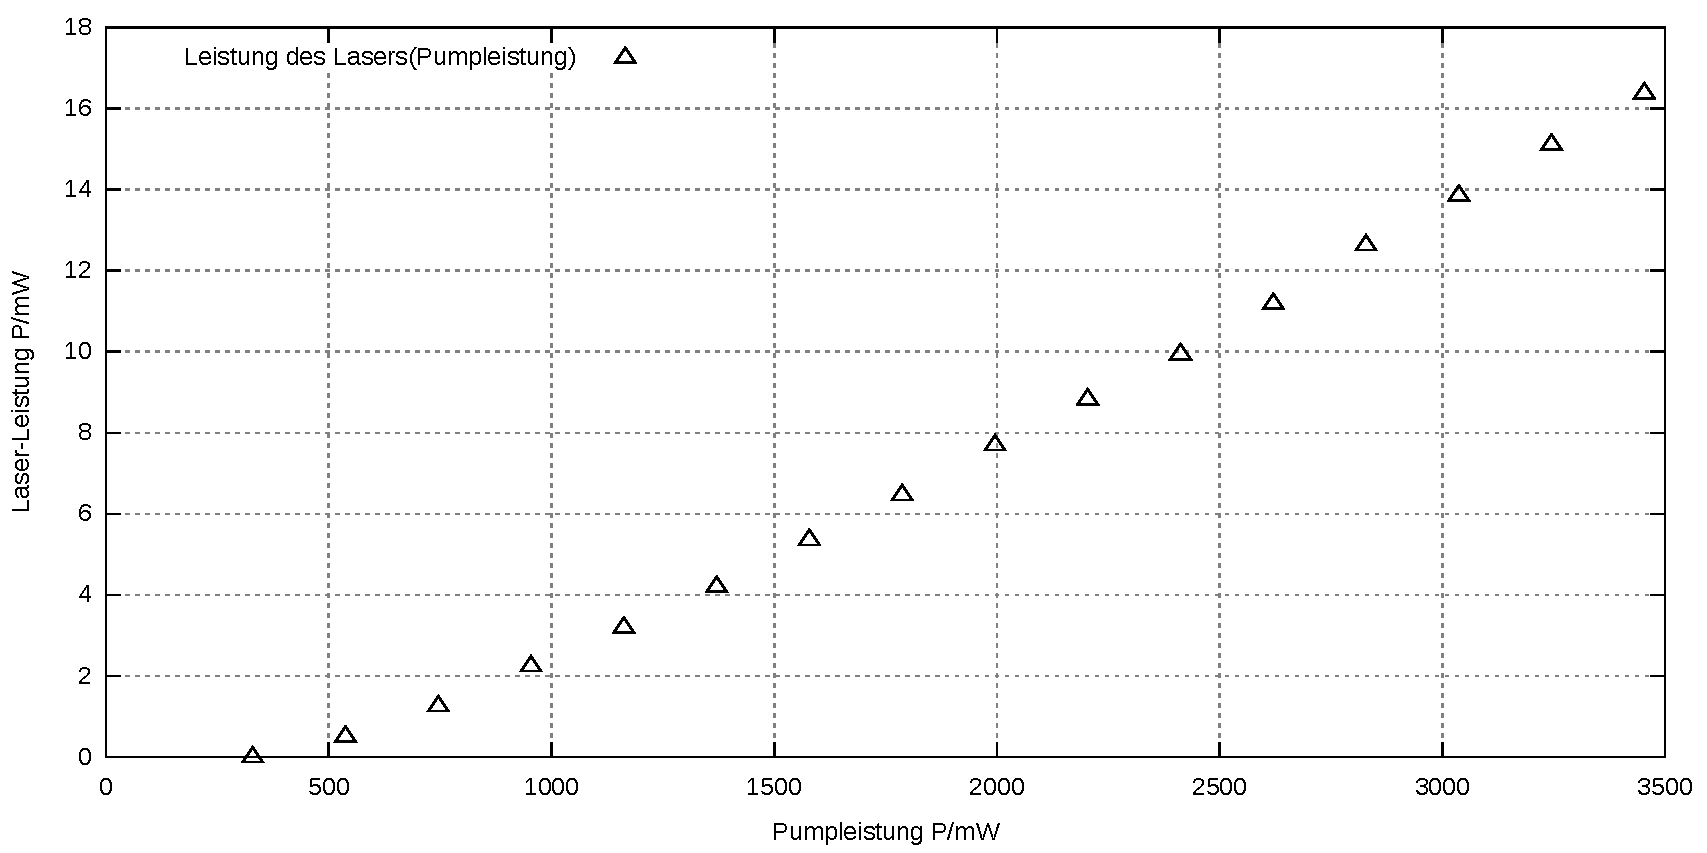
\includegraphics[width=\textwidth]{messwerte/laserleistung.pdf}
	\caption{Leistung des Lasers in Abhängigkeit der Pumpleistung bei konst. Temperatur}\label{img:grundwelle}
\end{figure}
Eine lineare Näherung (im geeigneten Bereich) lässt den Vergleich zwischen der Leistung der 1. Oberwelle in \ref{img:oberwelle} und der Grundwelle aus \ref{img:grundwelle} zu.\\
Für die Messung der 1. Oberwelle baut man in den Strahlengang des Lasers einen Kristall ein, dessen Eigenschaften gerade eine Frequenzverdopplung bei Durchgang einer elektromagnetischen Welle hervorrufen. Was damit schließlich im Detektor, nach Filterung des Pumpspektrums ankommt, ist die 1. Oberwelle der charakteristischen $\unit[1064]{nm}$-Linie, welche $\unit[532]{nm}$ entspricht. Die Strahlungsleistung dieser Welle sollte etwa $P\ix{2f}\sim P\ix{f}^2$ sein, d.h. quadratisch mit der Grundwellenleistung gehen.\\
Wie in \ref{img:oberwelle} und \ref{img:grundwelle} gut gesehen werden kann, können die Erwartungen bestätigt werden.
\begin{figure}[H]
 	\centering
 	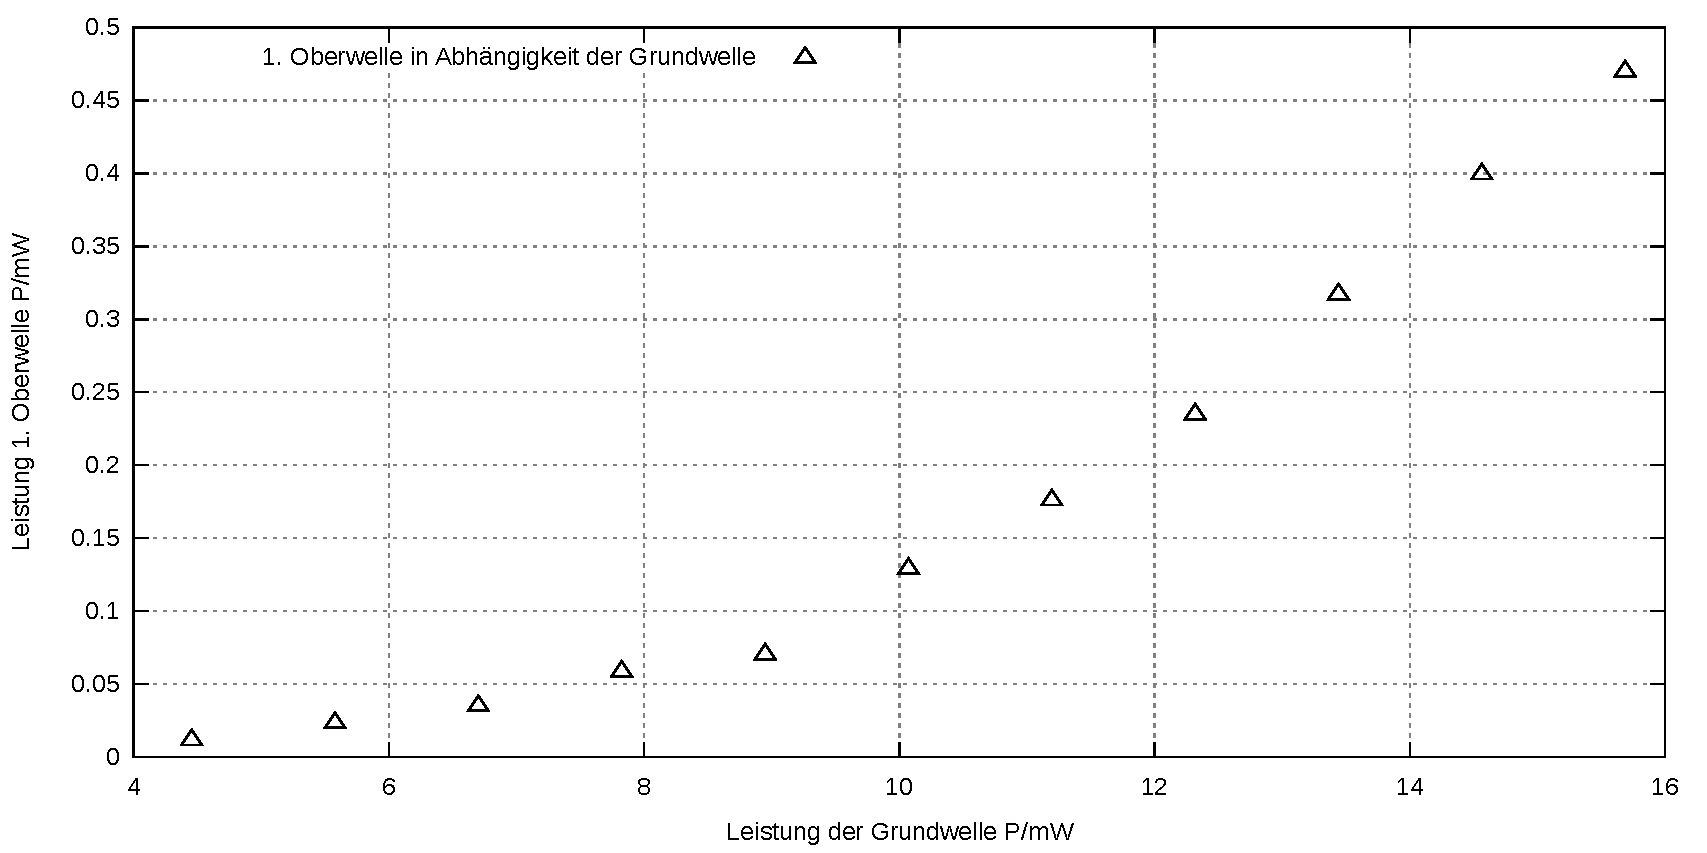
\includegraphics[width=\textwidth]{messwerte/lasergreun.pdf}
 	\caption{Leistung der 1. Oberwelle in Abhängigkeit der Leistung der Grundwelle}\label{img:oberwelle}
\end{figure}
\pagebreak
\section{Quellen}
	\url{http://de.wikipedia.org/wiki/Festk%C3%B6rperlaser}\newline\newline
	\url{http://de.wikipedia.org/wiki/Besetzungsinversion}\newline\newline
	\url{http://de.wikipedia.org/wiki/Laserdiode}\newline\newline
	\url{http://www.o-heinz.de/Deutsch/Hochschule/Download/Manual_L6.pdf}\newline\newline
	\url{http://www.dlf.ug.edu.pl/wp-content/uploads/2014/03/Miernik-mocy.pdf}\newline\newline
\end{document}